\documentclass{beamer}

\usepackage[utf8]{inputenc}
\usepackage[english,russian]{babel}
\usepackage{amsmath,amssymb, amsthm}
\usepackage{graphicx}
\usepackage{algorithm}
\usepackage{algpseudocode}
\usepackage{booktabs}
\usepackage{threeparttable}
\usepackage{colortbl}
\usepackage{pifont}
\usepackage{physics}
\usepackage{fontawesome5}
\usepackage[
    backend=biber,
    style=authoryear, 
    citestyle=authoryear,
    maxbibnames=99,
    language=english,
]{biblatex}
\DefineBibliographyStrings{russian}{
  andothers = {et\addabbrvspace al\adddot},
  in = {In},
  and = {and},
}
\addbibresource{ref.bib}

\newcommand{\cmark}{\textcolor{green!70!black}{\ding{51}}}
\newcommand{\xmark}{\textcolor{red}{\ding{55}}}

\usetheme{default}
\setbeamertemplate{navigation symbols}{}
\setbeamertemplate{footline}[frame number]
\setbeamertemplate{headline}{}

\theoremstyle{plain}
\newtheorem{assumption}{Предположение}

\title{Методы редукции дисперсии, не предполагающие вычисление полного градиента: повышение эффективности за счёт техники случайного перемешивания батчей}
\author[А.\,В.~Ребриков]{Алексей Витальевич Ребриков\\
\small{Научный руководитель: к.ф.-м.н. А.\,Н.~Безносиков}}
\institute{Кафедра интеллектуальных систем ФПМИ МФТИ\\
Специализация: Интеллектуальный анализ данных\\
Направление: 03.03.01 Прикладные математика и физика}
\date{2025}

\begin{document}

\begin{frame}
  \titlepage
\end{frame}

% Далее: строго структура как просил пользователь

\begin{frame}{Редукция дисперсии и полный градиент}

    \textbf{Проблема:} оптимизация конечной суммы:
    \[
    \min_{x\in\mathbb{R}^d} f(x) = \frac{1}{n}\sum_{i=1}^{n} f_i(x), 
    \quad f_i:\mathbb{R}^d \to \mathbb{R}, \quad n \gg 1.
    \]
    \vspace{-0.4em}
    \begin{itemize}
        \item GD: вычисляет полный градиент $\Rightarrow$ долго при большом $n$.
        \item SGD: не требует полного градиента $\Rightarrow$  дисперсия решения.
        \item Классические методы редукции дисперсии (VR, Variance Reduction) периодически вычисляют полный градиент.
    \end{itemize}
    \pause
    \only<2>{
    \vspace{0.5em}
    \begin{block}{Замечание}
        Стохастику ввели, чтобы избежать полного градиента, но в VR-методах к нему вернулись (хоть и реже)~--- \textcolor{red!85!black}{замкнутый круг}.
    \end{block}
    }
    \onslide<3->{
    \vspace{1.2em}
    \textbf{Цель:} Метод VR без вычисления полного градиента.\\
    \vspace{1.2em}
    \textbf{Решение:} Модификация алгоритма \texttt{SARAH}.\\
    Лучшие оценки сходимости~--- за счёт перемешивания батчей.
    }
    
\end{frame}

\begin{frame}{SARAH (StochAstic Recursive grAdient algoritHm)}
    Метод стохастической оптимизации с редукцией дисперсии.\\
    \vspace{1.2em}
    В отличие от \texttt{SGD} \textbf{рекурсивное обновление градиента}:
    \begin{itemize}
        \item уменьшает дисперсию оценок градиента без хранения всех,
        \item обходится редкими обращениями к полному градиенту.
    \end{itemize}

    \vspace{1.2em}
    \textbf{Алгоритм:}
    \begin{itemize}
        \item[$\blacktriangleright$] \textit{Начало эпохи:} $v^0 = \nabla f(x^0)$~--- полный градиент
        \item[$\blacktriangleright$] \textit{Внутри эпохи:}
        \[
        v^t = \nabla f_{i_t}(x^t) - \nabla f_{i_t}(x^{t-1}) + v^{t-1}, \quad 
        x^{t+1} = x^t - \gamma v^t
        \]
    \end{itemize}

    \vfill
    \scriptsize
    \faBook~\fullcite{nguyen2017sarah}
\end{frame}

\begin{frame}{Модификация SARAH: RR No Full Grad SARAH}
    \textbf{Алгоритм:}
        \begin{itemize}
            \item[$\blacktriangleright$] \textit{Начало эпохи:} 
            $v^0 = \mathbf{\tilde{v}^{n}}~\text{или начальная оценка (например, 0)}$
            \textit{где} $\mathbf{\tilde{v}^t}$~--- скользящая оценка полного градиента на шаге $t$
            
            \item[$\blacktriangleright$] \textit{Внутри эпохи:}
            \[
                v^t = \mathbf{\frac{1}{n}}\left(\nabla f_{i_t}(x^t) - \nabla f_{i_t}(x^{t-1})\right) + v^{t-1}, \quad 
                x^{t+1} = x^t - \gamma v^t
            \]
            \[
                \mathbf{\tilde{v}^{t+1}} = \frac{t-1}{t} \cdot \mathbf{\tilde{v}^{t}} + \frac{1}{t} \cdot \nabla f_{i_{t}}(x^{t}) 
            \]
        \end{itemize}
    \vspace{0.8em}
    \textbf{Особенности:}
    \begin{itemize}
        \item[$\blacktriangleright$] Перемешивание батчей~--- каждый ровно один раз за эпоху.
        \item[$\blacktriangleright$] Вместо полного градиента $v^0$ \textbf{скользящее среднее} $\mathbf{\tilde{v}}$.       
        \item[$\blacktriangleright$] \textbf{Домножение на $1/n$} $\Rightarrow$ дополнительно VR.
    \end{itemize}

    \vfill
    \scriptsize
    Первая идея исcледовалась в статье:\\
    \faBook~\fullcite{beznosikov2023random}
\end{frame}

\begin{frame}{Теоретические  результаты}
    Все $f_i$ — $L$-гладкие,\quad шаг $\gamma \le \frac{1}{20L(n+1)}$,\quad $n$ — размер выборки.\\
    \vspace{2em}
    \textbf{Невыпуклый случай:}
    \begin{align*}
        \varepsilon^2 &= \frac{1}{S} \sum_{s=1}^{S} \|\nabla f(x_s^0)\|^2 & \order{\frac{nL}{\varepsilon^2}} \\[1em]
        \intertext{\textbf{Cильно выпуклый случай:}}
        \varepsilon &= f(x_{S+1}^0) - f(x^*)  & \order{\frac{nL}{\mu} \log \frac{1}{\varepsilon}}
    \end{align*}
\end{frame}

    
    

% 4. Таблица сравнения
\begin{frame}{Предложенный алгоритм лучше красного}
    \centering
    \scriptsize
    \begin{tabular}{|c|c|c|c|c|}
    \hline
    \textbf{Алгоритм} & 
    \begin{tabular}{@{}c@{}}\textbf{Нет полного} \\ \textbf{градиента?}\end{tabular} & \textbf{Память} & \textbf{Невып.} & \textbf{Сильно вып.} \\
    \hline%
    SAGA & \cmark &  \(\order{\textcolor{red}{nd}}\) & --- & \(\order{n\frac{L^{\textcolor{red}{2}}}{\mu^{\textcolor{red}{2}}}\log\frac{1}{\varepsilon}}\) \\[1.52ex]
    \hline
    IAG & \cmark &  \(\order{\textcolor{red}{nd}}\) & --- & \(\order{n^{\textcolor{red}{2}}\frac{L^{\textcolor{red}{2}}}{\mu^{\textcolor{red}{2}}}\log\frac{1}{\varepsilon}}\) \\[1.52ex]
    \hline
    PIAG & \cmark &  \(\order{\textcolor{red}{nd}}\) & --- & \(\order{n\frac{L}{\mu}\log\frac{1}{\varepsilon}}\) \\[1.52ex]
    \hline
    DIAG & \cmark &  \(\order{\textcolor{red}{nd}}\) & --- & \(\order{n\frac{L}{\mu}\log\frac{1}{\varepsilon}}\) \\[1.52ex]
    \hline
    Prox-DFinito & \cmark & \(\order{\textcolor{red}{nd}}\) & --- & \(\order{n\frac{L}{\mu}\log\frac{1}{\varepsilon}}\) \\[1.52ex]
    \hline
    AVRG & \cmark &  \(\order{d}\) & --- & \(\order{n\frac{L^{\textcolor{red}{2}}}{\mu^{\textcolor{red}{2}}}\log\frac{1}{\varepsilon}}\) \\[1.52ex]
    \hline
    SVRG  & \xmark &  \(\order{d}\) & --- & \(\order{n^{\textcolor{red}{3}}\frac{L^{\textcolor{red}{2}}}{\mu^{\textcolor{red}{2}}}\log\frac{1}{\varepsilon}}\) \\[1.52ex]
    \hline
    SVRG & \xmark &  \(\order{d}\) & \(\order{\frac{nL}{\varepsilon^2}}\) & \(\order{n\frac{L^{\textcolor{red}{3/2}}}{\mu^{\textcolor{red}{3/2}}}\log\frac{1}{\varepsilon}}\) \\[1.52ex]
    \hline
    SARAH  & \cmark & \(\order{d}\) & --- & \(\order{n^{\textcolor{red}{2}}\frac{L}{\mu}\log\frac{1}{\varepsilon}}\) \\[1.52ex]
    \hline
    \rowcolor{gray!10}RR NFG SARAH  & \cmark & \(\order{d}\) & \(\order{\frac{nL}{\varepsilon^2}}\) & \(\order{n\frac{L}{\mu}\log\frac{1}{\varepsilon}}\) \\[1.52ex]
    \hline
    \end{tabular}
\end{frame}

% \begin{scope}
% % 5. CIFAR-10 эксперимент
% \begin{frame}{Эксперимент: CIFAR-10 + ResNet18}
%     Рассматривается задача многоклассовой классификации на датасете CIFAR-10, 
%     \begin{itemize}
%         \item 60\,000 изображений размером $32\times32$
%         \item 10 классов (по 6\,000 изображений на класс)
%     \end{itemize} 
    
%     Используется классическая архитектура модели ResNet-18

%     Оптимизируется стандартная функция потерь~--- кросс-энтропия:
%     \[
%     \min\limits_{w} \frac{1}{M} \sum_{i=1}^{M} \ell(f_w(x_i), y_i),
%     \]
%     где $w$~--- параметры модели, $f_w(x_i)$~--- предсказание модели на входе $x_i$, $y_i$~--- истинная метка, $\ell$~--- кросс-энтропия.
%     \end{frame}
    

% % 6. Графики
% \begin{frame}{Графики}
% \begin{figure}
% \centering    
% 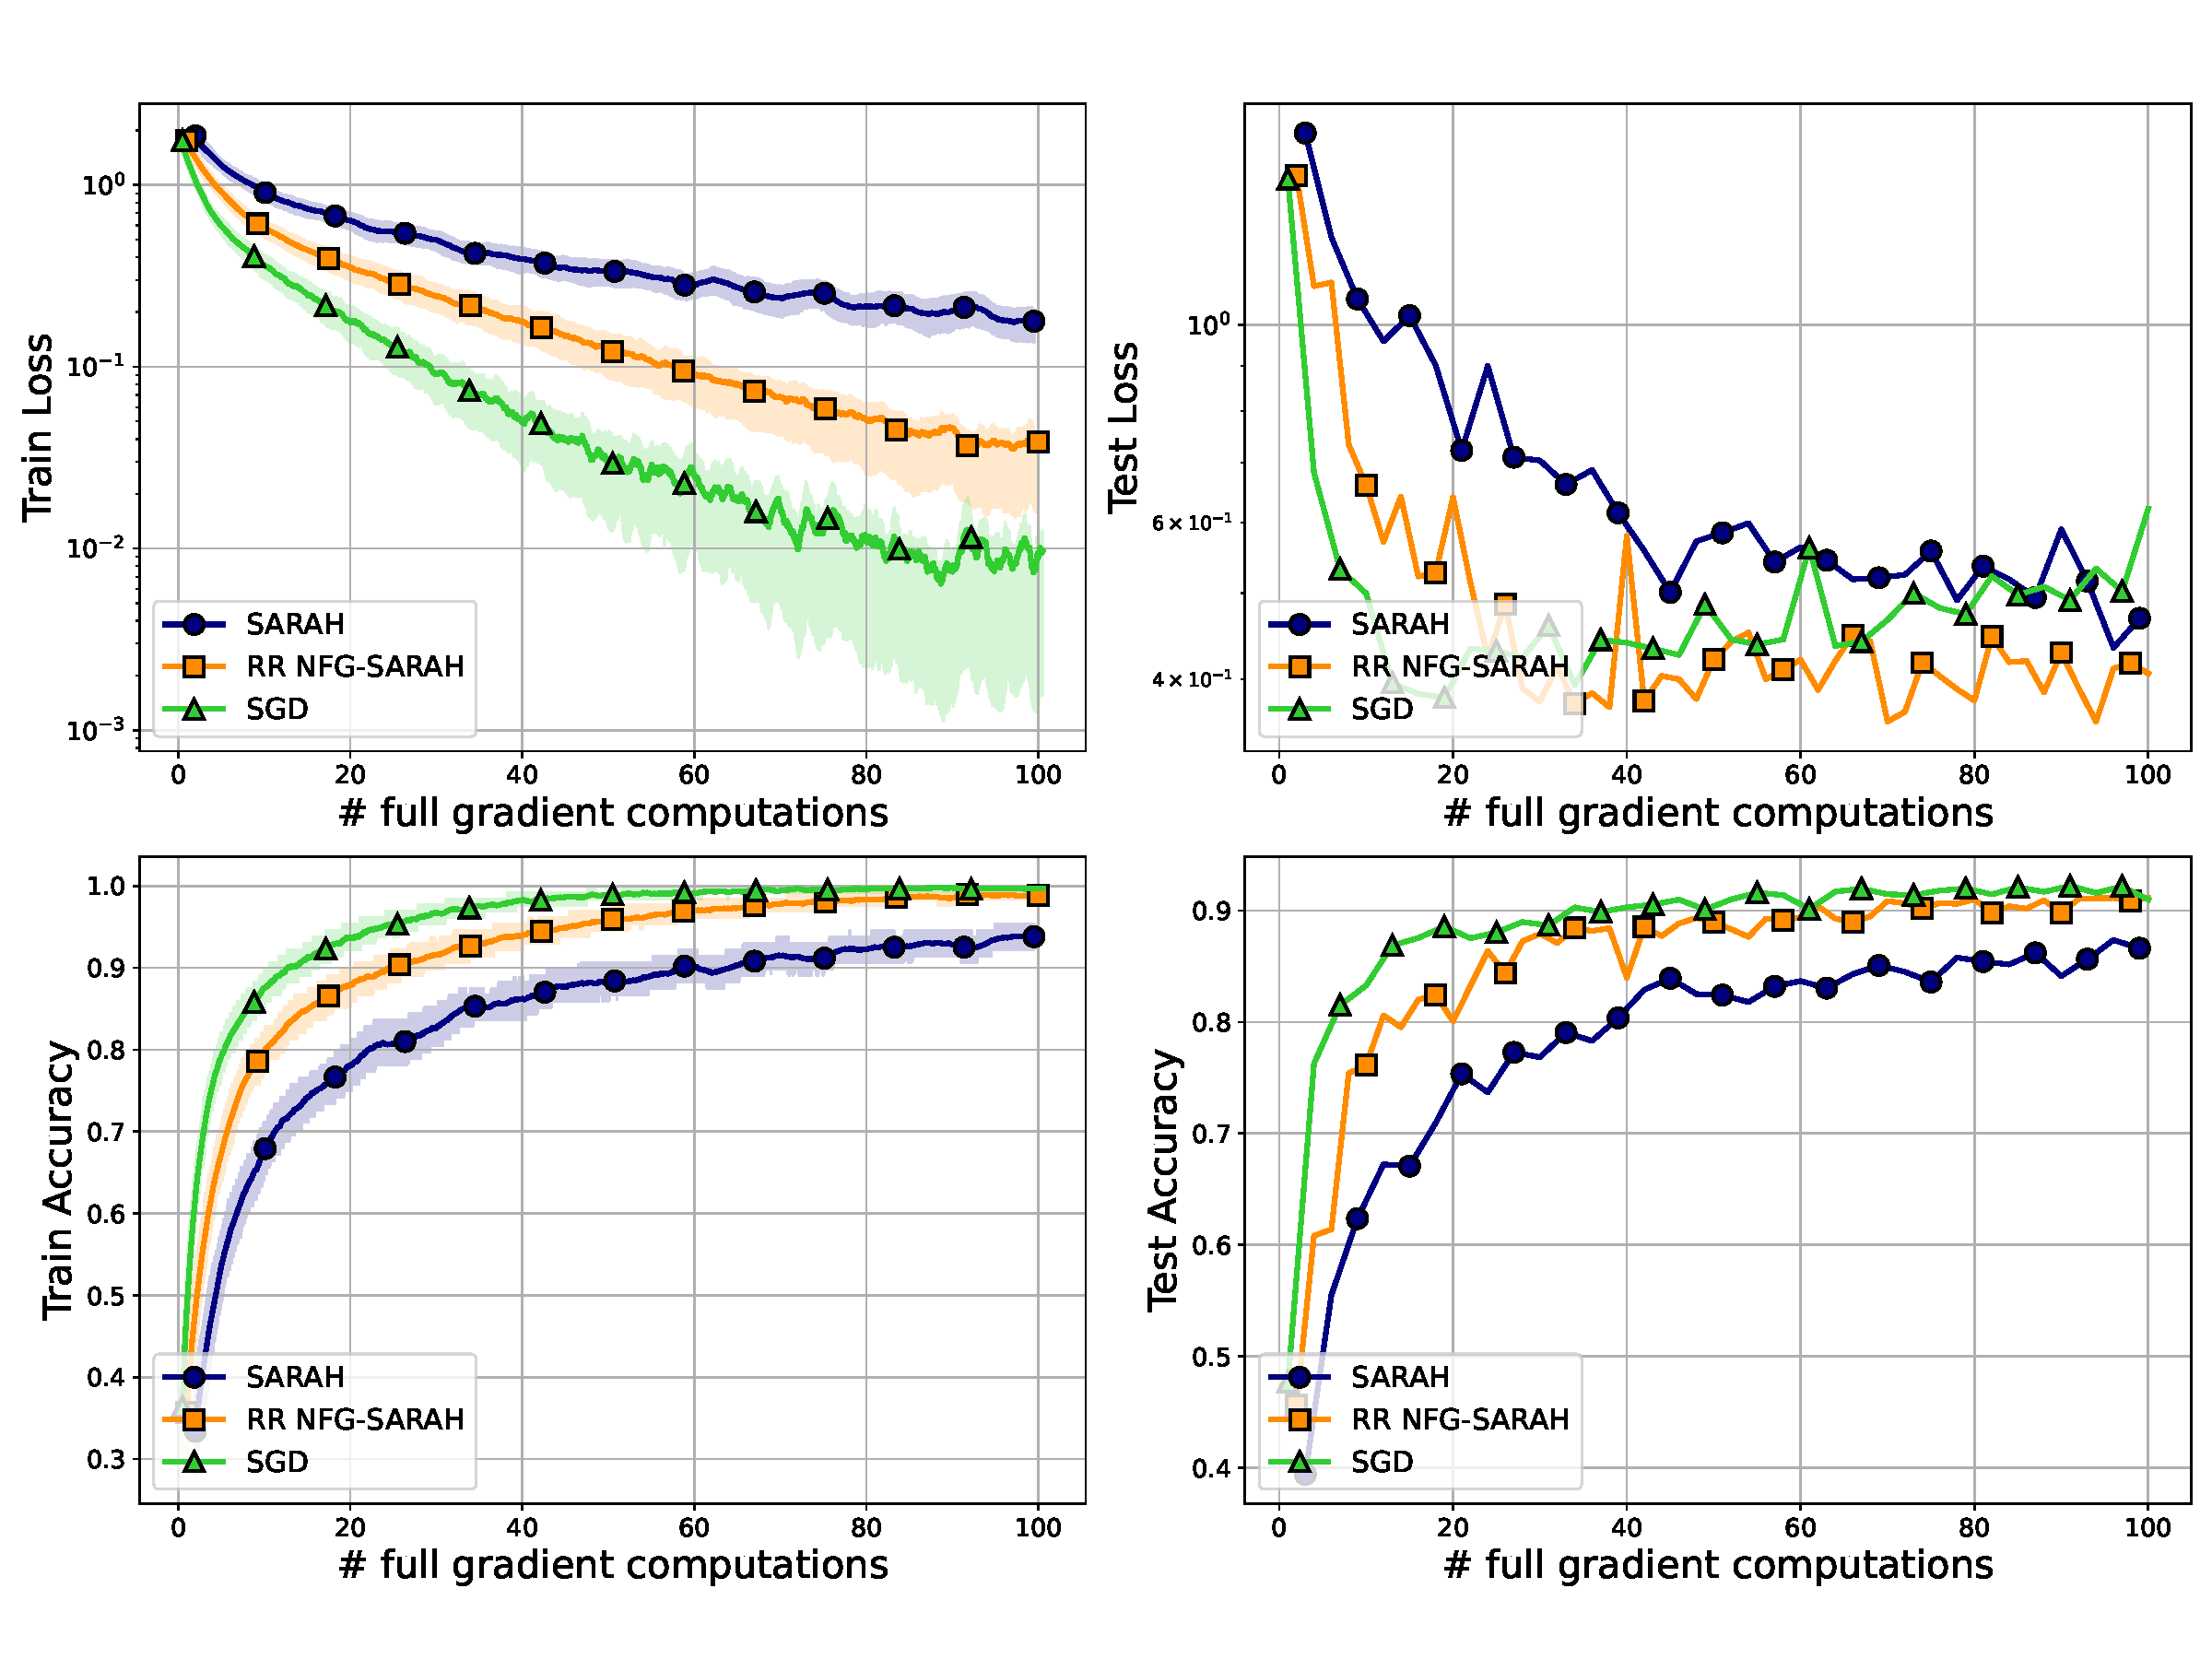
\includegraphics[width=\linewidth]{../figures/sarah_10.pdf}
% \end{figure}
% \end{frame}

% \begin{frame}{Эксперимент: CIFAR-100 + ResNet18}
%     Задача многоклассовой классификации на датасете CIFAR-100:
%     \begin{itemize}
%         \item 60\,000 изображений $32\times32$
%         \item 100 классов (по 600 изображений на класс)
%     \end{itemize}

%     Используется архитектура ResNet-18.

%     Функция потерь~--- кросс-энтропия:
%     \[
%     \min\limits_{w} \frac{1}{M} \sum_{i=1}^{M} \ell(f_w(x_i), y_i),
%     \]
%     где $w$~--- параметры модели, $f_w(x_i)$~--- выход модели, $y_i$~--- метка, $\ell$~--- кросс-энтропия.

%     Метод \textsc{No Full Grad SARAH} сравнивается с классическим \textsc{SARAH}.
% \end{frame}

% \begin{frame}{Графики: CIFAR-100}
% \begin{figure}
% \centering
% 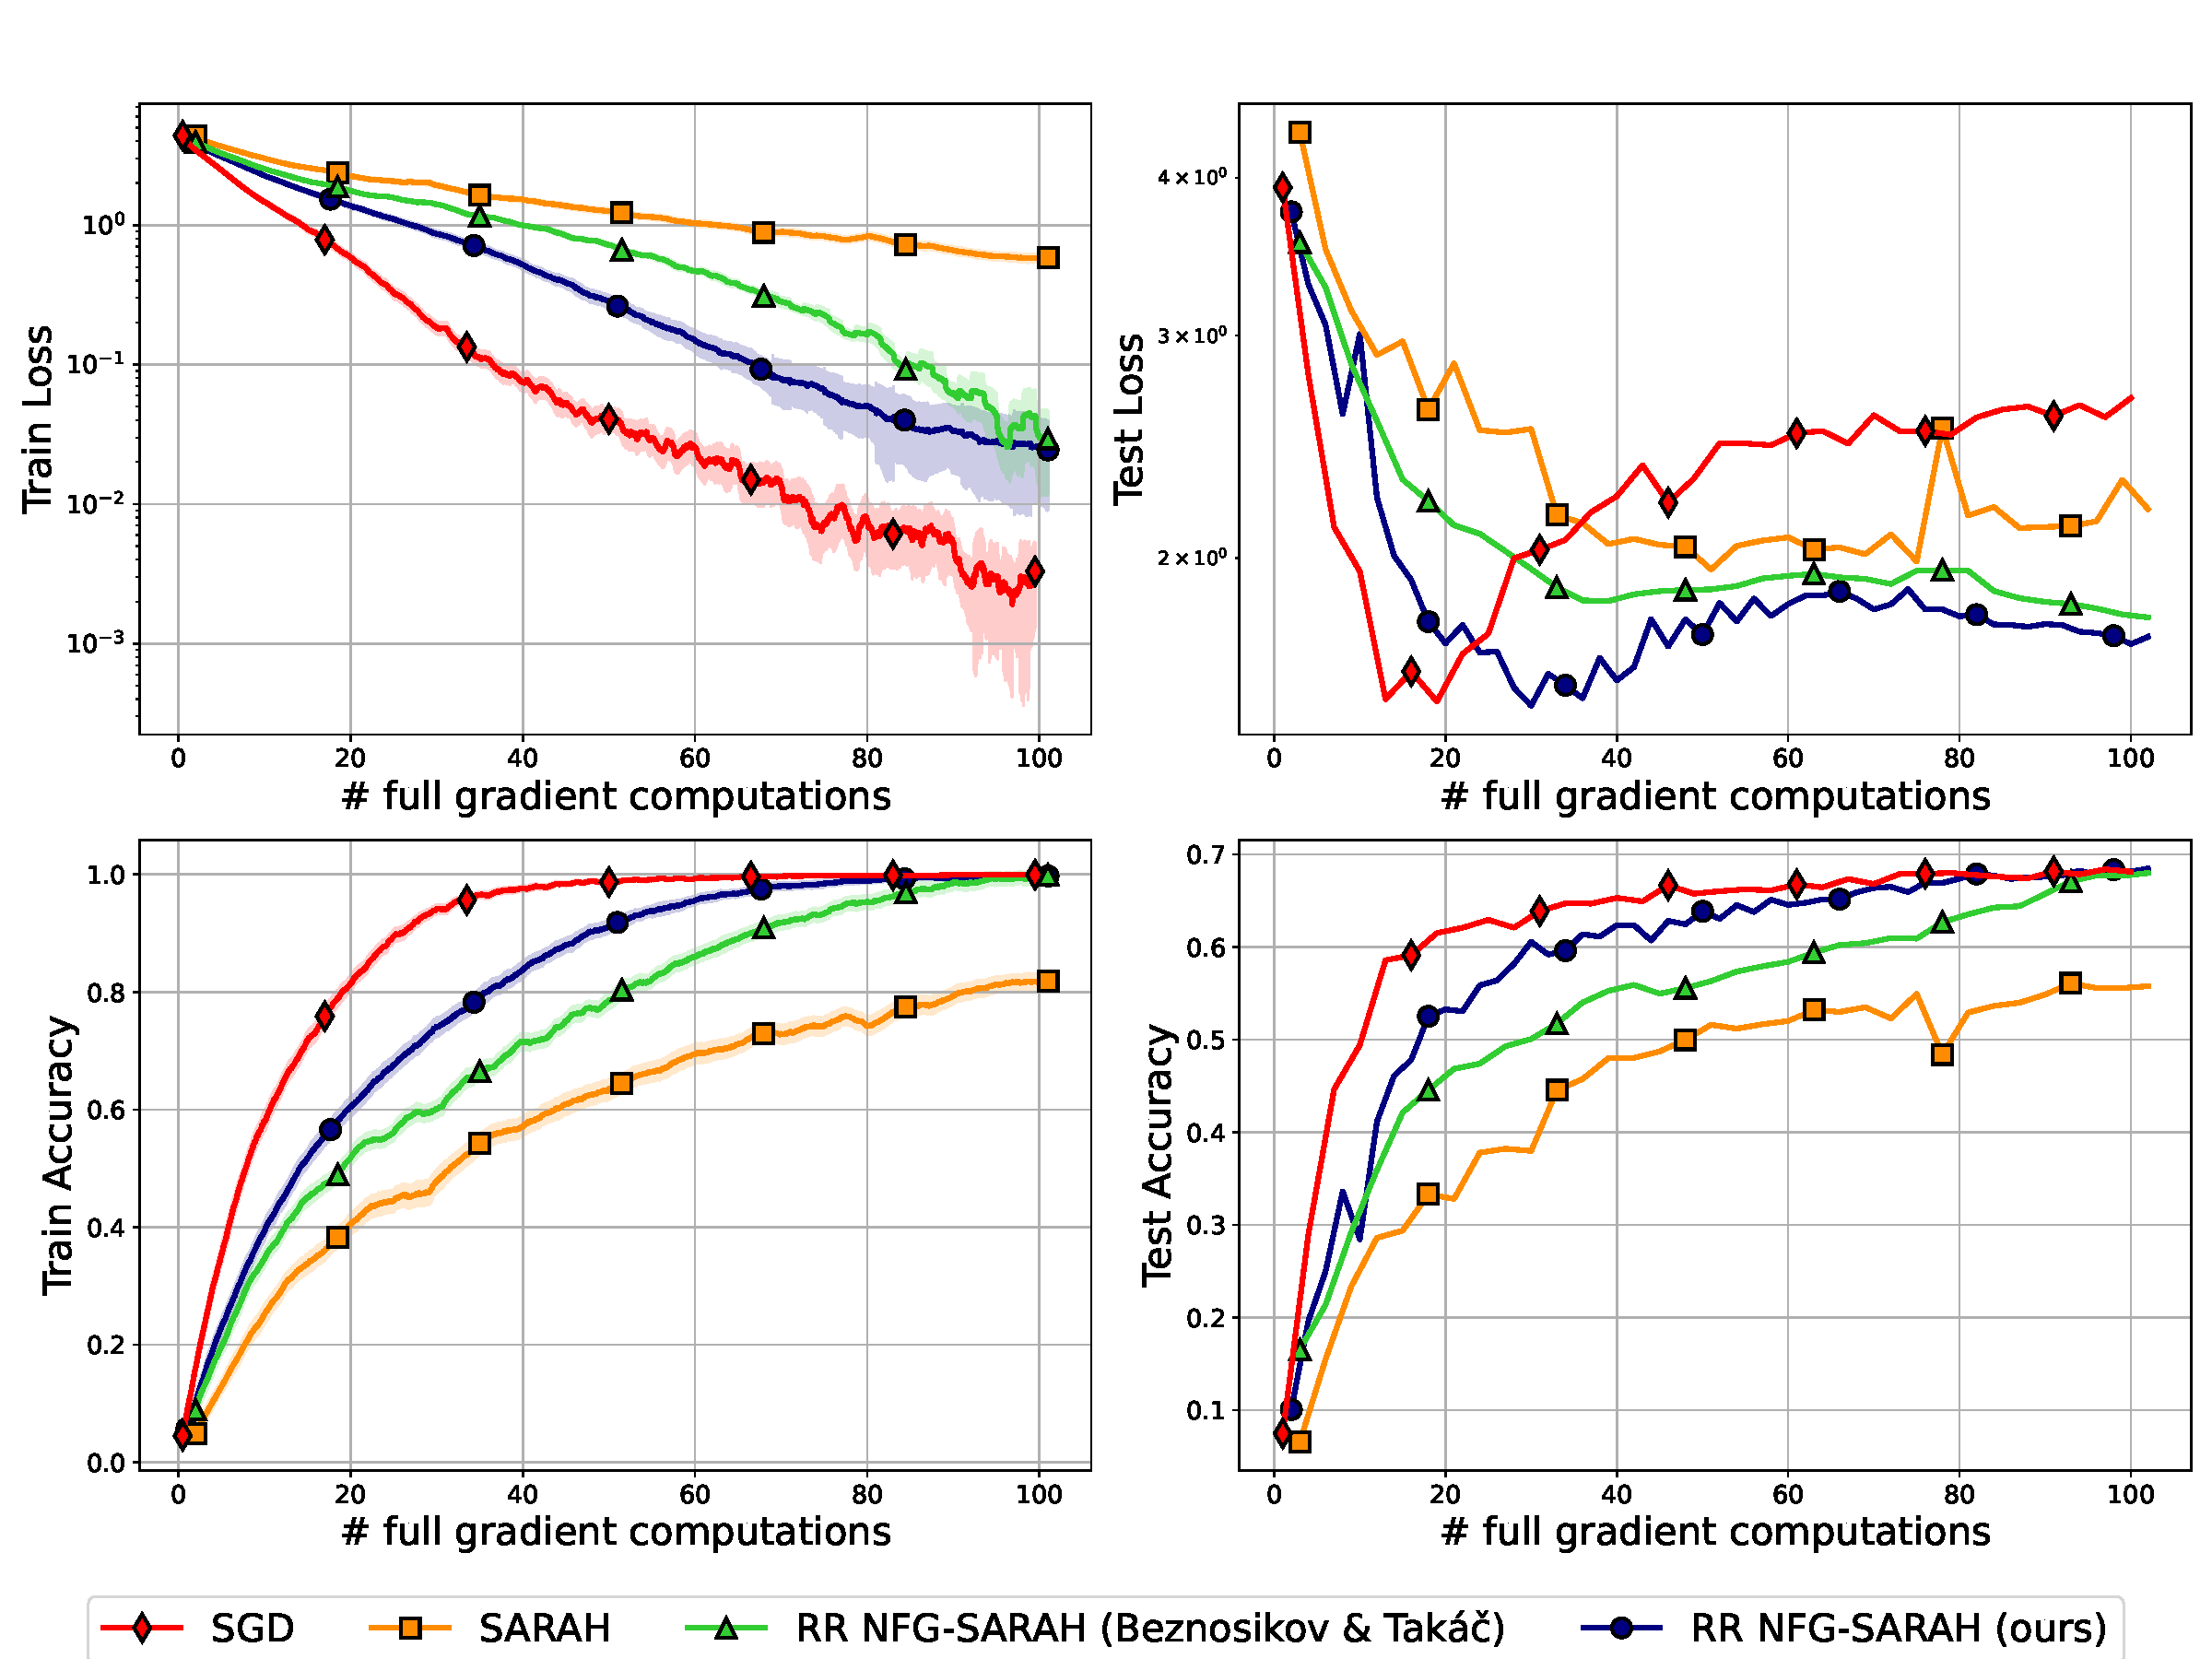
\includegraphics[width=\linewidth]{../figures/CIFAR100_LR=0.7_plots_compressed.pdf}
% \end{figure}
% \end{frame}

% \begin{frame}{Эксперимент: Tiny ImageNet + Swin Transformer}
%     Задача классификации изображений на Tiny ImageNet:
%     \begin{itemize}
%         \item 200 классов, изображения $64\times64$
%         \item масштабирование до $224\times224$ для Swin
%     \end{itemize}

%     Используется модель Tiny Swin Transformer (\texttt{swin\_T\_patch4\_window7\_224}), инициализированная предобученными весами с ImageNet-1K.

%     Размер батча: 256, градиентный клиппинг: 1.0. Метрики: точность и кросс-энтропия. Сравниваются методы: \textsc{SGD}, \textsc{SARAH}, RR \textsc{NFG-SARAH}, предложенный \textsc{No Full Grad SARAH}.
% \end{frame}

% \begin{frame}{Графики: Tiny ImageNet}
% \begin{figure}
% \centering
% 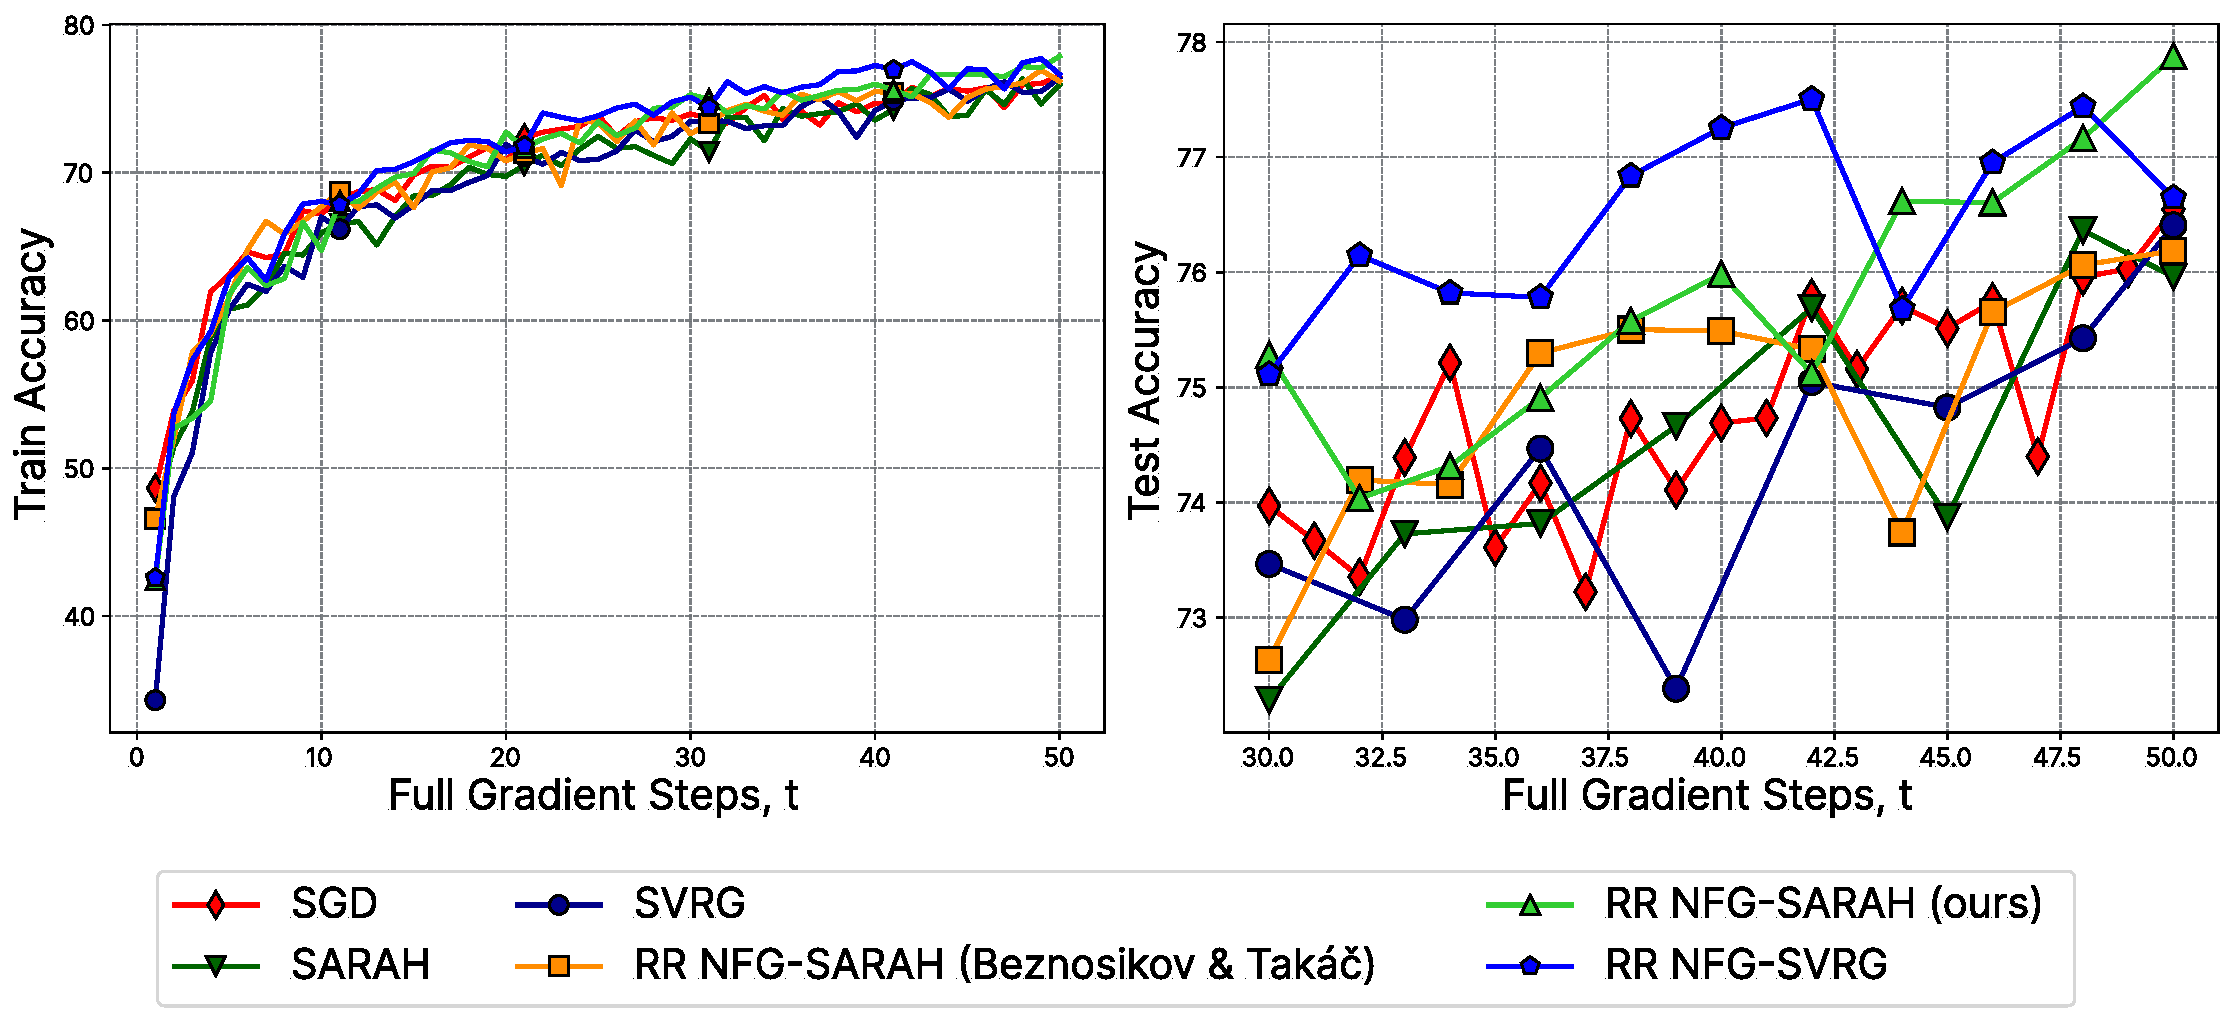
\includegraphics[width=\linewidth]{../figures/vit_results.pdf}
% \end{figure}
% % \begin{table}
% % \centering
% % \begin{tabular}{l|c}
% % \toprule
% % Метод & Точность ($\uparrow$) \\
% % \midrule
% % \textsc{SGD} & 76.545 \\
% % \textsc{SARAH} & 75.961 \\
% % RR \textsc{NFG-SARAH} () & 76.186 \\
% % RR \textsc{NFG-SARAH} (предложенный) & \textbf{77.875} \\
% % \bottomrule
% % \end{tabular}
% % \end{table}
% \end{frame}
% \end{scope}

\begin{frame}{Эксперимент: CIFAR-10 + ResNet18}
    Многоклассовая классификация на CIFAR-10:
    \begin{itemize}
        \item 60\,000 изображений $32\times32$ в 10 классах
        \item Архитектура: ResNet-18
        \item Функция потерь: кросс-энтропия
        \[
        \min\limits_{w} \frac{1}{M} \sum_{i=1}^{M} \ell(f_w(x_i), y_i)
        \]
        \item Метрики: точность и кросс-энтропия
        \item Все методы сравниваются по числу эквивалентных вызовов полного градиента
    \end{itemize}
    \vfill
    \scriptsize
    Подробности эксперимента на CIFAR-100 см. в работе.
\end{frame}

\begin{frame}{Сходимость на CIFAR-10 (ResNet-18)}
    \centering
    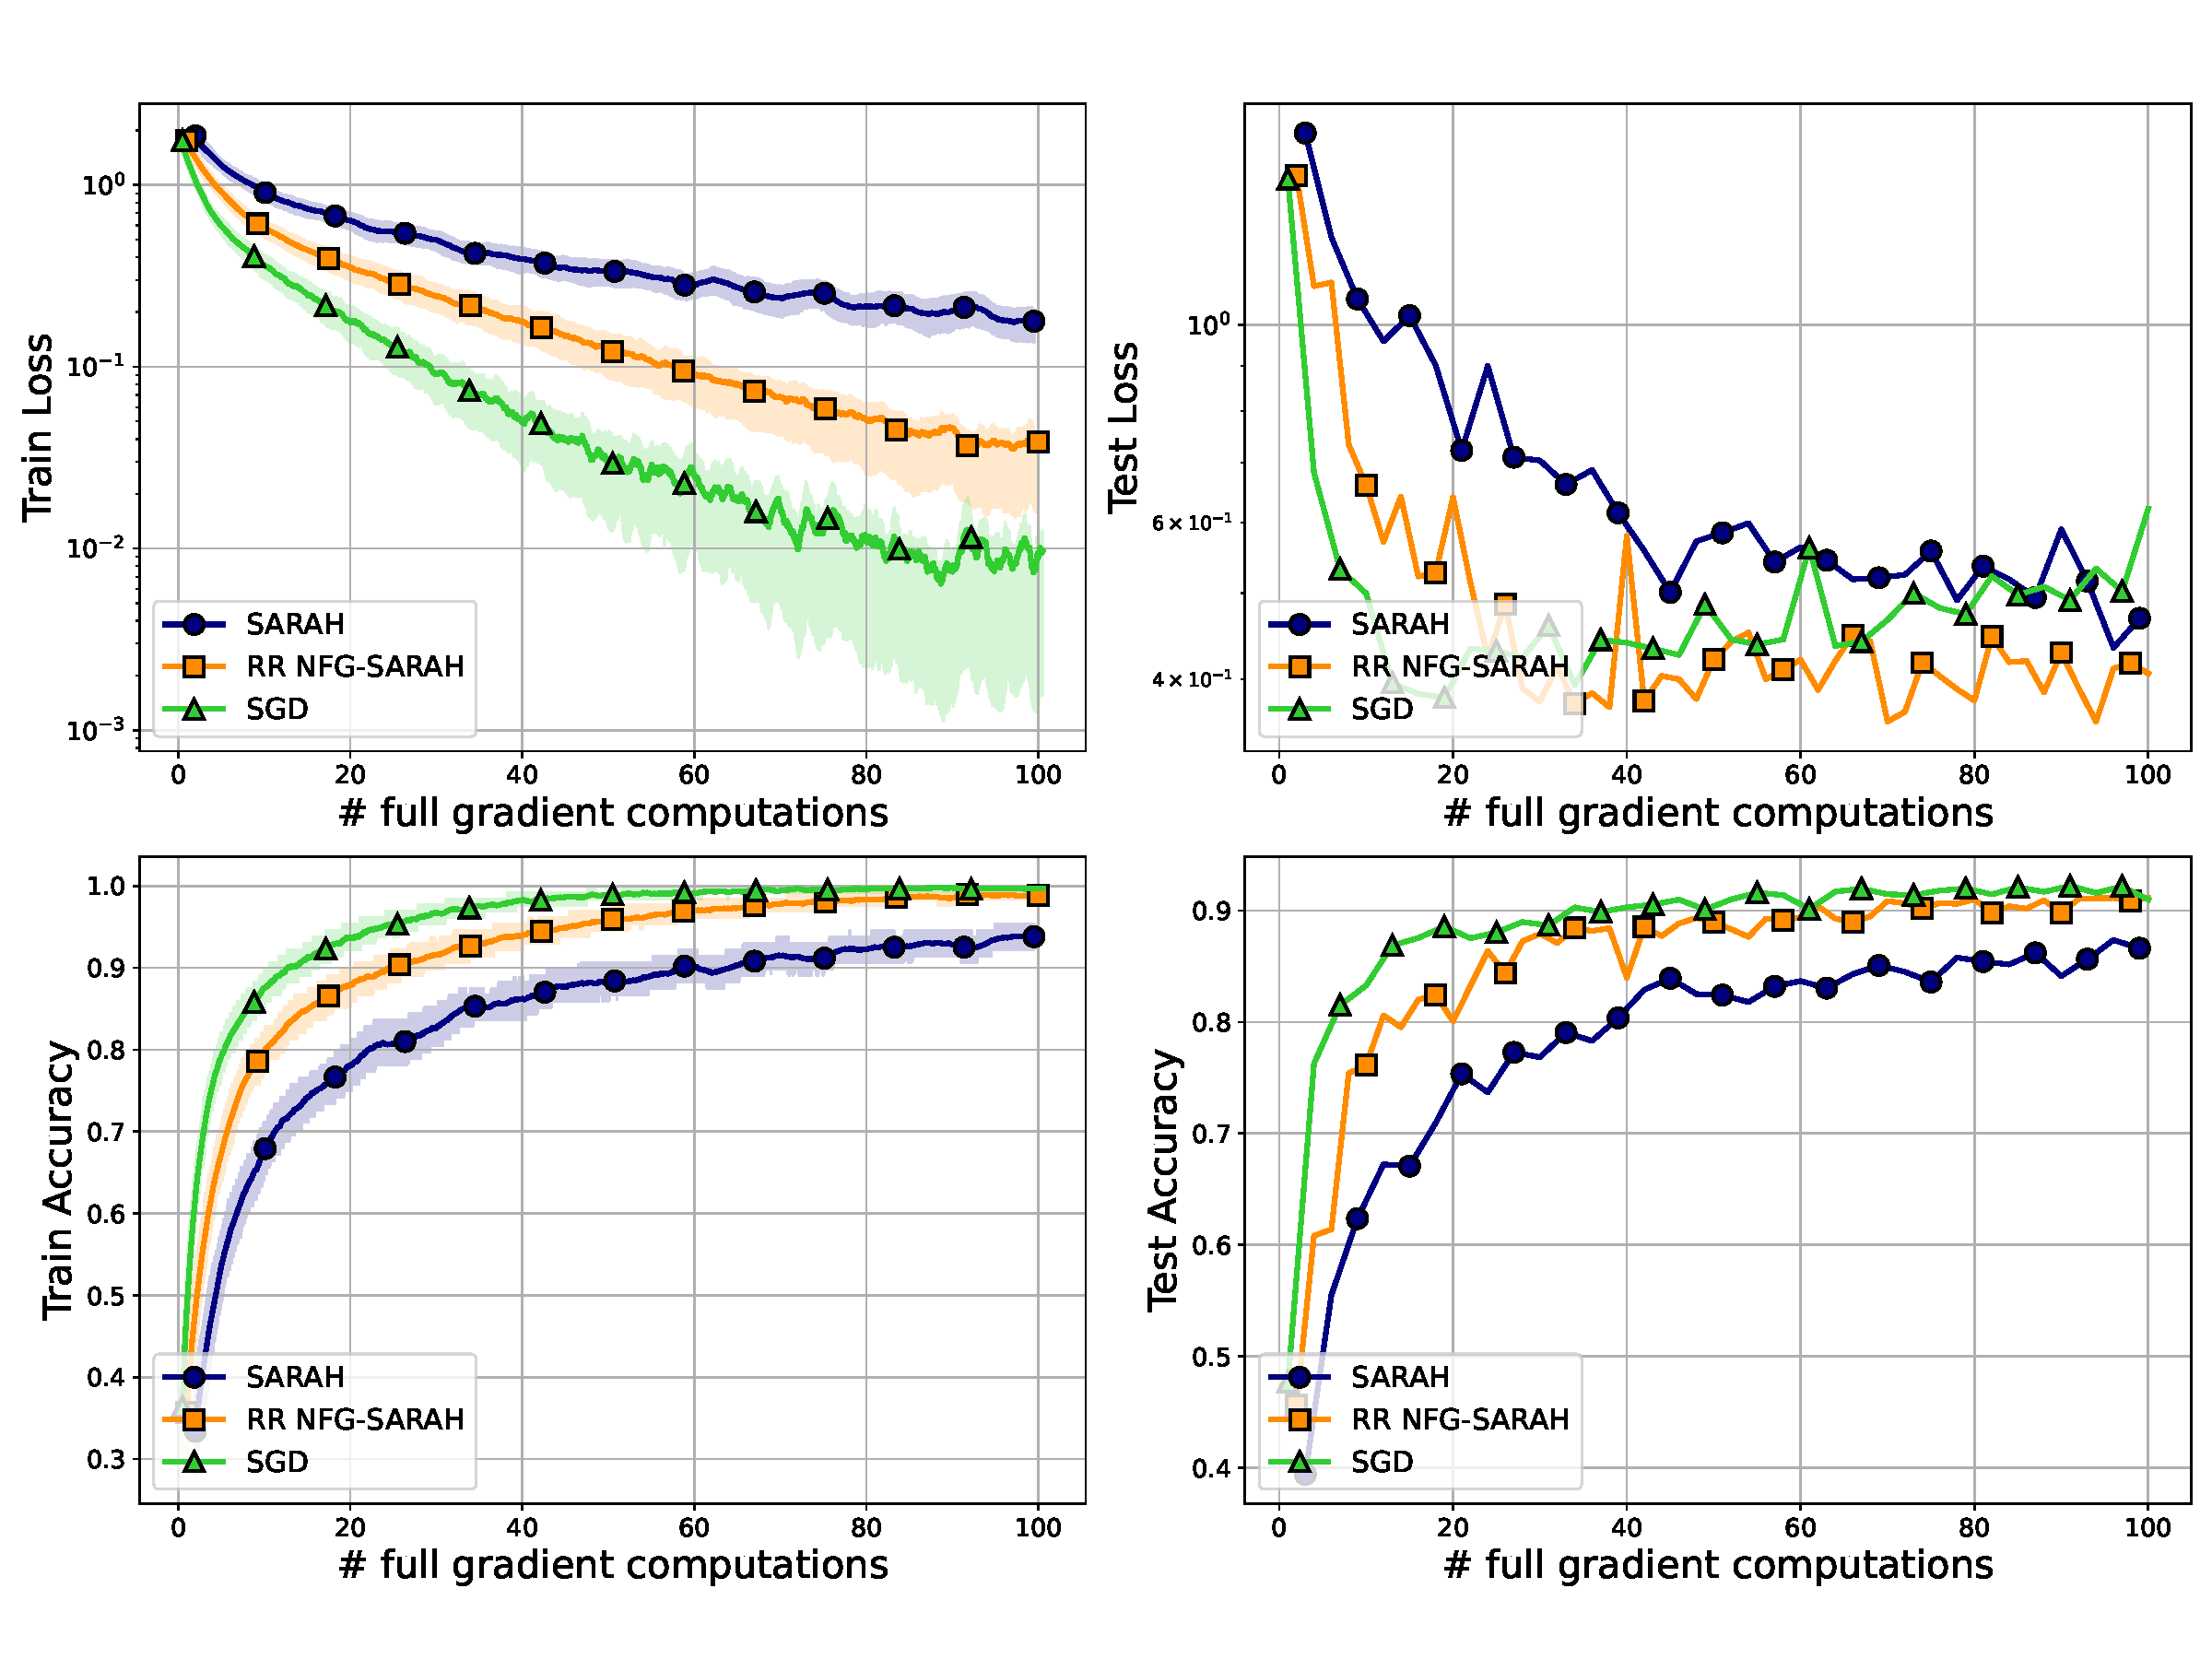
\includegraphics[width=0.9\linewidth]{../figures/sarah_10.pdf}
    \scriptsize\\
    Везде сравнимо или лучше, чем \texttt{SGD}. Везде лучше, чем \texttt{SARAH}.
\end{frame}


\begin{frame}{Эксперимент: Swin Transformer + Tiny ImageNet}
    Многоклассовая классификация изображений:
    \begin{itemize}
        \item Tiny ImageNet: 200 классов, $64\times64$, масштаб до $224\times224$
        \item Модель: Tiny Swin Transformer (\texttt{swin\_T\_patch4\_window7\_224}) с предобучением на ImageNet-1K
        \item Функция потерь: кросс-энтропия
        \[
        \min\limits_{w} \frac{1}{M} \sum_{i=1}^{M} \ell(f_w(x_i), y_i)
        \]
        \item Метрики: точность и кросс-энтропия
        \item Все методы сравниваются по числу эквивалентных вызовов полного градиента
    \end{itemize}
\end{frame}

\begin{frame}{Сходимость на  Tiny ImageNet (Swin Transformer)}
    \begin{center}
    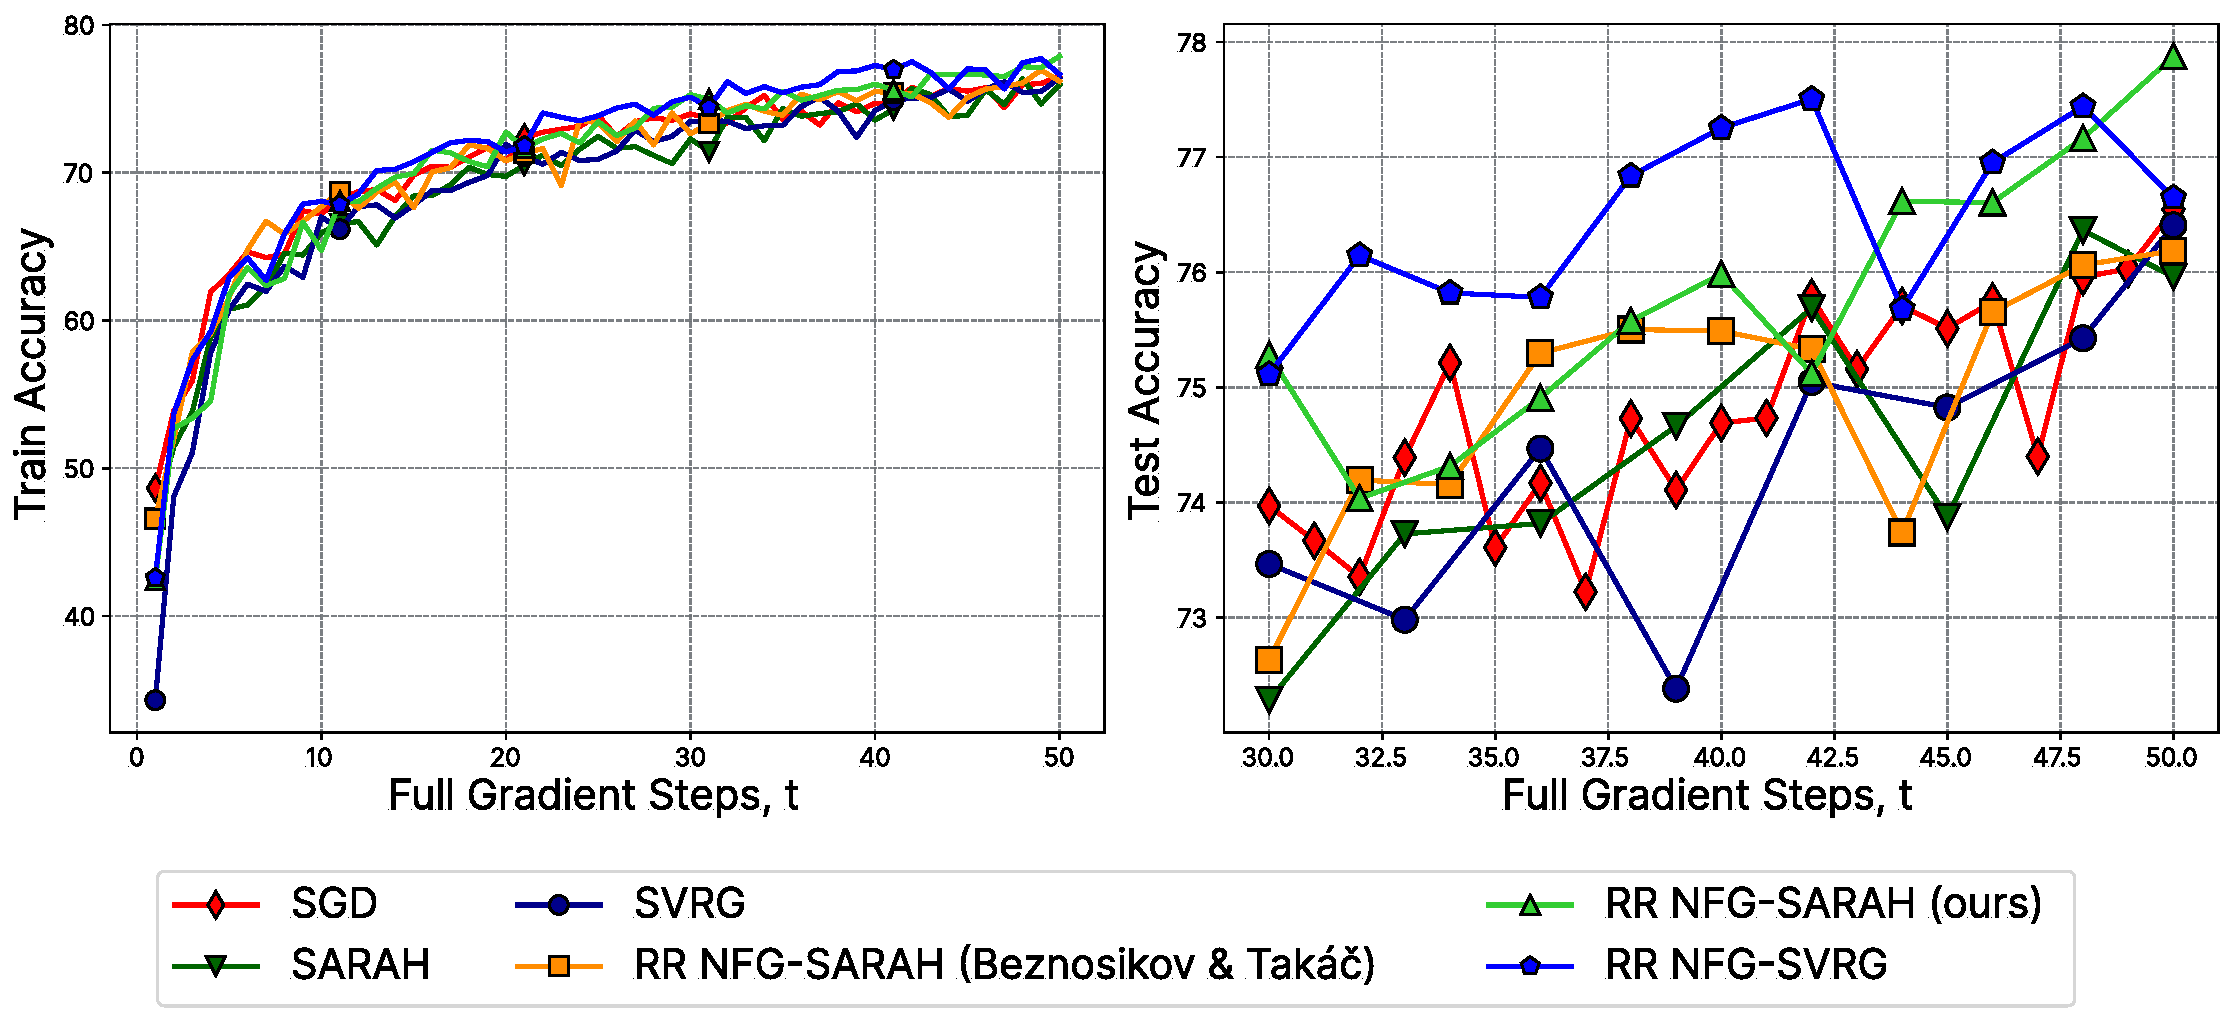
\includegraphics[width=\linewidth]{../figures/vit_results.pdf}
    \scriptsize
    Предложенный метод достигает лучшей точности. Сходимость на тестовой выборке стабильнее остальных.
    \end{center}
    \vspace{1em}
    \scriptsize
    Дополнительно приведен алгоритм из статьи (упоминалась на 4 слайде):\\
    \faBook~\fullcite{beznosikov2023random}
\end{frame}

    
\begin{frame}{Выносится на защиту}
    \begin{itemize}
        \item Разработан новый вариант метода \textbf{SARAH}, не использующий вычисление полного градиента.
        \item За счёт перемешивания и скользящего среднего достигается аппроксимация полного градиента без дополнительного хранения.
        \begin{itemize}
            \item \textbf{Память:} требуется \(\order{d}\) вместо \(\order{nd}\)
            \item \textbf{Сходимость:} улучшенные оценки по числу итераций
        \end{itemize}
        \item Проведена серия экспериментов (CIFAR-10/CIFAR-100 с ResNet-18, Tiny ImageNet с Swin Transformer), подтверждающих теоретические результаты.
        \item Работа была представлена на 67-й Всероссийской научной конференции МФТИ.
        \item Полученные результаты объединены с другими исследованиями и поданы в виде статьи на международную конференцию уровня A* в области машинного обучения.
    \end{itemize}
\end{frame}



    
\end{document}
